\section{Method}

In this section I outline the method I used to forecast upper limits for PMF detection using mock stage-3 and stage-4 covariance matrices and simulated CMB power spectra. In section 3.1 I will introduce the Fisher matrix, its properties and discuss how it is useful for experimental design. In section 3.2 I will discuss how I obtained CMB power spectra and how they are used to construct the Fisher matrix. Next, in section 3.3 I will describe the properties of the mock covariances and how I processed them into a useable format. Finally in section 3.4 will bring all the pieces together and explain how to obtain a Fisher matrix, apply conditioning to secure it against numerical instabilities and apply a change of variables to recieve forecasts for the upper limits on $B_{1Mpc}$.

\subsection{Introduction to Fisher Matrices}
The elements of the Fisher matrix are defined as:
\begin{equation}
\mathcal{F}_{ij} = - \left \langle \frac{\partial^{2}ln{\mathcal{L}}}{\partial p^i\partial p^j } \right \rangle
\end{equation}
where $\mathcal{L}$ is the likelihood and $p^{i}$, $p^{j}$ are the $i^{th}$ and $j^{th}$ model parameters.
\\\\
If the Fisher matrix is non-singular then it can be inverted into a covariance matrix for the model parameters. This result follows from the Cram\`{e}r-Rao theorem, which states that the variance of some unbiased estimator, p is greater than or equal to the inverse of its Fisher information. The Fisher information of a model parameter is given by:

\begin{equation}
F = - \langle \frac{\partial^{2}ln{\mathcal{L}}}{{\partial p}^2} \rangle
\end{equation}

Since the Fisher matrix can be inverted into a covariance matrix over the model parameters, it is a powerful tool in experimental design used for forecasting the upper limits on the precision of an experiment. The Fisher matrix has a number of useful properties:

Firstly, it is linear under addition: Adding n Fisher matrices returns a new Fisher matrix which can be inverted into a new covariance matrix with tighter constraints. This result is especially useful when you wish to know the total accuracy of many combined experiments.
\begin{equation}
(\mathcal{F}_{1} + \mathcal{F}_{2} + ... + \mathcal{F}_{n})^{-1} = \mathcal{F}^{-1}_{1+2+...+n}
\end{equation}

As a corollary, the Fisher matrix can be multiplied by a scalar, which is useful when you want to know the effect of repeating your experiment or adding more instances of the same design.

Furthermore, one can use this property to add priors to your design: suppose we know that one model parameter has been well-constrained in the past and our experiment isn't set to improve upon this result. We can combine the prior result with our current Fisher matrix to provide tighter constraints, like so:

$$ \begin{bmatrix}
F_{aa} & F_{ab} & F_{ac}\\ 
F_{ba} & F_{bb} & F_{bc} \\ 
F_{ca} & F_{cb} & F_{cc}
\end{bmatrix}
+
\begin{bmatrix}
0 & 0 & 0\\ 
0 & 0 & 0 \\ 
0 & 0 & P
\end{bmatrix} $$

Here, we have a prior, P on variable c. All we need to do is add P to the corresponding diagonal term. However, if the prior is too big the Fisher matrix becomes singular. To combat this we employ the second useful property of Fisher matrices, marginalisation.

If we have a Fisher matrix with more variables than we're interested in, we can just throw away the rows and columns associated with the variables that we don't care about. The resultant matrix is a Fisher matrix that is valid for the remaining variables - there's no need to recalculate the Fisher matrix with fewer variables!

Returning to the case where P $>>$ $F_{cc}$, we can marginalise over the variable c by removing its associated rows and columns from the Fisher matrix. In this case the information lost is negligible, since the variance from our experiment was much larger than P's experiment anyway. In return, we now find we can forecast for the remaining variables.

Usually, the Fisher matrix is found by calculating the log-likelihood for the model parameters. This is done by making likelihood chains in Markov-chain-Monte-Carlo simulations however this is not the only approach. If your model parameters are unbiased and Gaussian distributed then the following definition for the Fisher matrix holds:

\begin{equation}
F_{ij} = \frac{\partial f}{\partial p^i} C^{-1} \frac{\partial f}{\partial p^j}
\end{equation}

where $f$ is the function that relates the model parameters to each other, $C$ is the covariance matrix for(???) and $p^{i}$ are the model parameters. In this thesis I will take $f$ to be the CMB polarisation power spectrum, $C_{\ell}$. Next, ${p}$ will be the $\Lambda CDM$ parameters as well as some additional parameters (see 3.X) and finally $C$ are mock covariance matrices associated with CMB-S3-like and CMB-S4-like experiments. Equation (12) then becomes:

\begin{equation}
F_{ij} = \frac{\partial C_{\ell}}{\partial p^i} C^{-1} \frac{\partial C_{\ell}}{\partial p^j}
\end{equation}

\subsection{CMB power spectra}

To begin constructing the Fisher matrix in the form given by (12), I first used CAMB to build the CMB power spectrum. [describe CAMB] [also cite CAMB]

To call on CAMB one first needs to define parameters. A quick summary of the parameters and their central values is given in table 2. The parameters I varied were the six $\Lambda CDM$ model parameters: $\Omega_{b}h^{2}$, the baryonic density. $\Omega_{c}h^{2}$, the cold dark matter density. $H_0$, Hubble's constant. $\tau$, the optical depth of reionisation. $\tau$ is a measure of approximately when reionisation occurred. $n_s$, the scalar spectral index for the primordial power spectrum, given by $P(k) = A_s k^{n_s - 1}$. $A_s$ is the amplitude of the primordial power spectrum. In addition we also have: The running of the scalar index, $n_{run}$. The effective number of neutrinos, $N_{eff}$ and the tensor-to-scalar ratio, $r$, which is used in constraining the effects of primordial gravity waves.

\begin{table}[h]
\centering
\caption{CAMB Parameters and Values}
\label{my-label}
\begin{tabular}{l|l|l|l}
Parameter & \multicolumn{1}{c|}{Value} & Uncertainty & Step Size \\ \hline
$\Omega_{b}h^{2}$ & \multicolumn{1}{c|}{0.02227716} & \multicolumn{1}{c|}{0.00023} & \multicolumn{1}{c}{$\pm 8 \times 10^{-5}$} \\
$\Omega_{c}h^{2}$ & \multicolumn{1}{c|}{0.1184293} & \multicolumn{1}{c|}{0.022} & \multicolumn{1}{c}{$\pm 10^{-3}$} \\
$H_0$ & \multicolumn{1}{c|}{67.86682} & \multicolumn{1}{c|}{0.96} & \multicolumn{1}{c}{$\pm 8 \times 10^{-2}$} \\
$\tau$ & \multicolumn{1}{c|}{0.06664549} & \multicolumn{1}{c|}{0.019} & \multicolumn{1}{c}{$\pm 10^{-3}$} \\
$n_s$ & \multicolumn{1}{c|}{0.9682903} & \multicolumn{1}{c|}{0.0062} & \multicolumn{1}{c}{$\pm 10^{-3}$} \\
$A_s$ & \multicolumn{1}{c|}{2.140509e-09} & \multicolumn{1}{c|}{0.118} & \multicolumn{1}{c}{$\pm 9 \times 10^{-12}$} \\
$n_{run}$ & \multicolumn{1}{c|}{0.0} & \multicolumn{1}{c|}{-} & \multicolumn{1}{c}{$\pm 2 \times 10^{-3}$} \\
$N_{eff}$ & \multicolumn{1}{c|}{3.03066666667} & \multicolumn{1}{c|}{0.23} & \multicolumn{1}{c}{$\pm 4 \times 10^{-3}$} \\
$r$ & \multicolumn{1}{c|}{0.01} & \multicolumn{1}{c|}{-} & \multicolumn{1}{c}{$\pm 8 \times 10^{-4}$} \\
\end{tabular}
\bigskip
\\This table shows the 6 $\Lambda CDM$ model parameters, as well as the running of the scalar index, the effective number of neutrinos and the tensor-to-scalar ratio. The 'Value' column shows the central value I entered into CAMB when producing the polarisation power spectrum and the 'Step Size' column indicates the magnitude of the perturbation around the central value I used for calculating the numerical derivatives. Finally, the 'Uncertianty' column gives the PLANCK best fit (2015) \cite{Ade:2015xua} $\Lambda CDM$ uncertainties, which were used as an upper bound for step sizes.
\end{table}
\\

In order to differentiate the power spectrum as required by (12) I employ a numerical form of the derivative:

\begin{equation}
\frac{\partial C_{\ell}}{\partial p} \approx \frac{\Delta C_{\ell}}{\Delta p}
\end{equation}
\\
Where $\Delta C_{\ell} = C^{upper}_{\ell} - C^{lower}_{\ell}$ and $\Delta p = p^{upper} - p^{lower}$. To calculate $\Delta C_{\ell}$ I call two instances of CAMB. In the first instance I add small perturbations to the central values (see table 2). The output power spectrum is called $C^{upper}_{\ell}$. The second instance, $C^{lower}_{\ell}$ has small perturbations subtracted from the central values. Finally, $\Delta p$ is equal to two times the perturbation values given in table 2.

To ensure that the derivatives are accurate the step sizes must be small, however if the step size is too small, the derivatives are subject to numerical artifacts. To choose well-conditioned step sizes I isolated each variable and generated a set of $\Delta C_{\ell}$s while holding all other parameters fixed and varying the step size. To compare the step sizes I then plotted each family of $\Delta C_{\ell}$. When choosing a step size I looked for two things:

\begin{enumerate}
\item Convergence: As the step size approaches the best value, $\Delta C_{\ell}$ will lose sensitivity to changes in step-size and the functions will converge to the same values for all $\ell$.

\item Smoothness: If the step size is too small then $\Delta C_{\ell}$ will oscillate significantly over a short change in $\ell$. The resultant plot will look 'blocky' or have large spikes and won't resemble a well-conditioned derivative of the CMB power spectrum.
\end{enumerate}

As a final sanity check on the value of the step sizes, I would like them to be less than the 2015 PLANCK best fit uncertainties (refer to table 2).
\\
Figure 7 shows a plot of $\Delta C_{\ell}$ for the BB polarisation power spectrum, varying Hubble's constant and holding all else fixed. The top panel shows the differences over $ 0 < \ell < 5000$. The lines all appear to be converging on the same function. The blue line, corresponding to a step size of 0.02 has significant artifacting, so by criterion one it can be ruled out. The second panel is zoomed in on the peak and trough over $\ell ~ 700$. Taking a closer look at the lines reveals that as the step size increases toward 0.1 the lines begin to converge. There isn't an ostensible difference between step sizes of 0.08 or 0.1, so the deciding factor is which one produces a better approximation of $\frac{\partial C_{\ell}}{\partial p}$. Smaller step sizes suit this purpose so for Hubble's constant I chose 0.08.

\begin{figure}
\centering
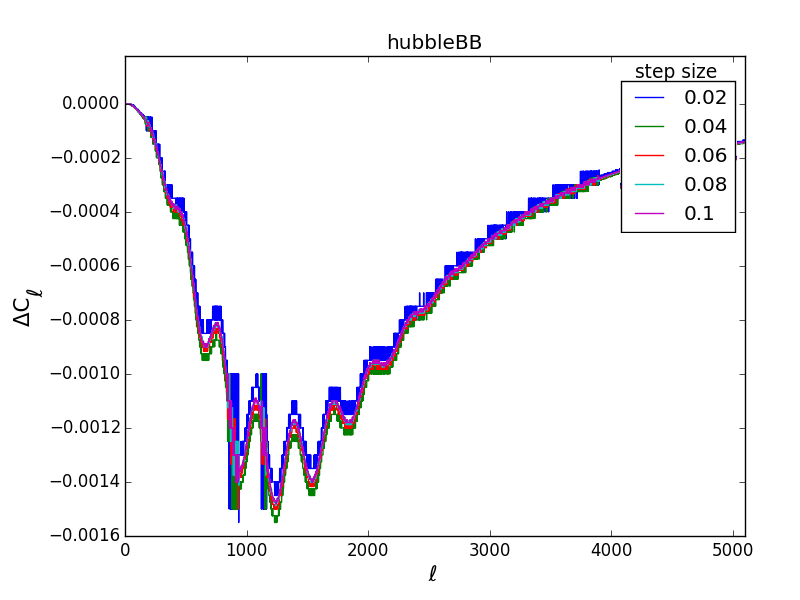
\includegraphics[scale=0.6]{images/diffs/H0bb.png}
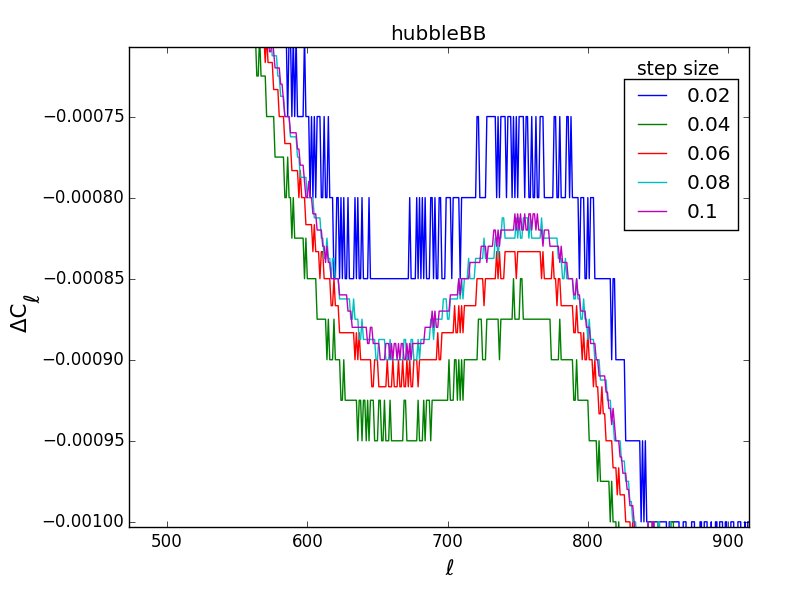
\includegraphics[scale=0.6]{images/diffs/H0bbz.png}
\caption{placeholder}
\end{figure}
\\
An interesting second case is the difference plot for the tensor-to-scalar ratio. When $\ell < 220$ the difference plot is well behaved with good convergence and few artifacts for larger step sizes. When $\ell > 220$ numerical effects begin to dominate.

\begin{figure}
\centering
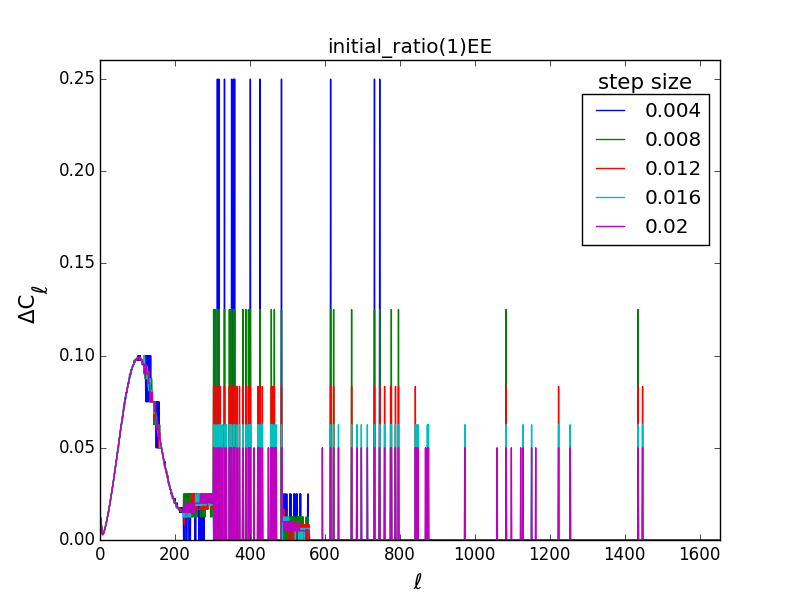
\includegraphics[scale=0.75]{images/diffs/reez.png}
\caption{placeholder}
\end{figure}

\subsection{Covariance Matrix}

For the inverse covariance matrix in (12) I used mock stage-3 and stage-4-like covariance matrices. These covariance matrices were calculated as per Tegmark (1997) \cite{Tegmark:1997vs} and model five experimental parameters: Scan area, noise, $\ell_{knee}$, beam width and beam error. The values for these parameters match up with various stage-3 and stage-4 experimental designs.
Scan area is the area of sky that these experiments will observe given in square degrees. For reference SPT-3G will observe a $2500 deg^{2}$ patch of sky whereas PLANCK observed the whole sky.
Noise is the background/instrumental(?) noise level of the experiment. This parameter is directly related to the number of bolometers in the experiment.

\subsection{Constructing the Fisher Matrix}
\subsection{tests}
